\section{Parameter Efficiency with CNNs}

\subsection{CNN Implementation}

\begin{itemize}
    \item Final validation accuracy: \textbf{99.03\%}
    \item Number of parameters: \textbf{421,642}
    \item Training time: \textbf{4.8 minutes}
\end{itemize}

\begin{figure}[h]
    \centering
    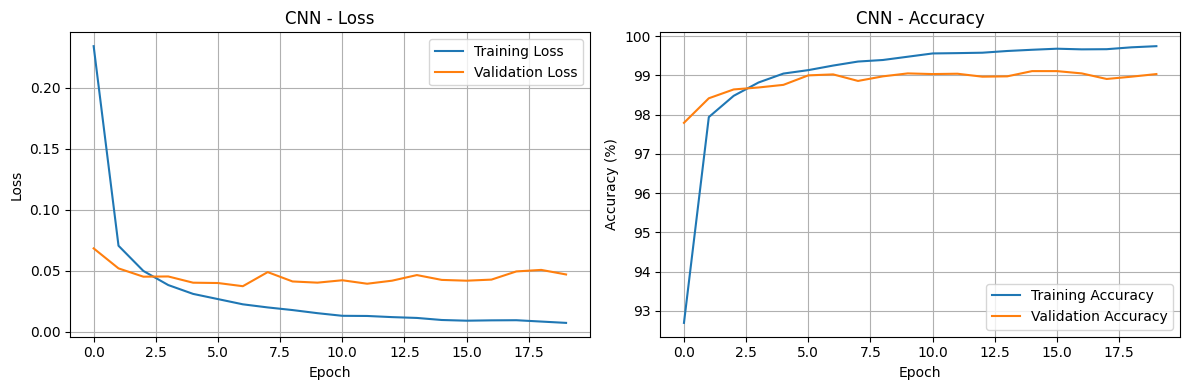
\includegraphics[width=0.7\linewidth]{section3/cnn.png}
    \caption{Training and validation curves for CNN model}
    \label{fig:cnn}
\end{figure}

\subsection{Question 3.1: Parameter Comparison}

\begin{table}[h]
\centering
\begin{tabular}{|l|c|c|c|}
\hline
\textbf{Model} & \textbf{Parameters} & \textbf{Val Acc} & \textbf{Train-Val Gap} \\ \hline
MLP (Dropout) & 535,818 & 98.31\% & 1.08\% \\ \hline
CNN & 421,642 & 99.03\% & 0.77\% \\ \hline
\end{tabular}
\caption{CNN vs MLP comparison}
\label{tab:cnn-comparison}
\end{table}

The CNN has 21.3\% fewer parameters (114,176 reduction) than the MLP.

\subsection{Question 3.2: Why do CNNs perform better?}

Despite having fewer parameters, the CNN achieves superior validation accuracy (99.03\% vs 98.31\%) with minimal overfitting. CNNs are better suited for image data because:

\begin{enumerate}
    \item \textbf{Spatial structure preservation}: Convolutional layers maintain 2D spatial relationships between pixels, while MLPs flatten images and destroy this information.
    
    \item \textbf{Translation invariance}: Weight sharing allows CNNs to recognize patterns regardless of position—a digit in any corner is recognized equally well.
    
    \item \textbf{Parameter efficiency}: Convolutional filters share weights across spatial locations. A 3×3 filter with 32 channels needs only 288 parameters, versus 25,088 for an equivalent fully-connected layer.
    
    \item \textbf{Hierarchical features}: CNNs learn low-level features (edges) in early layers and combine them into high-level features (shapes, objects) in deeper layers, mimicking human vision.
\end{enumerate}

The CNN demonstrates clear superiority: 21.3\% fewer parameters, 0.72\% higher accuracy, and better generalization (0.77\% train-val gap vs 1.08\% for MLP).